\documentclass[10pt]{article}
\usepackage{tikz}
\usetikzlibrary{shapes.misc}
\usepackage[margin=0cm]{geometry}
\pagestyle{empty}
\tikzstyle{every node}=[cross out, draw, red]

\begin{document}

\vspace*{\fill}
\begin{center}
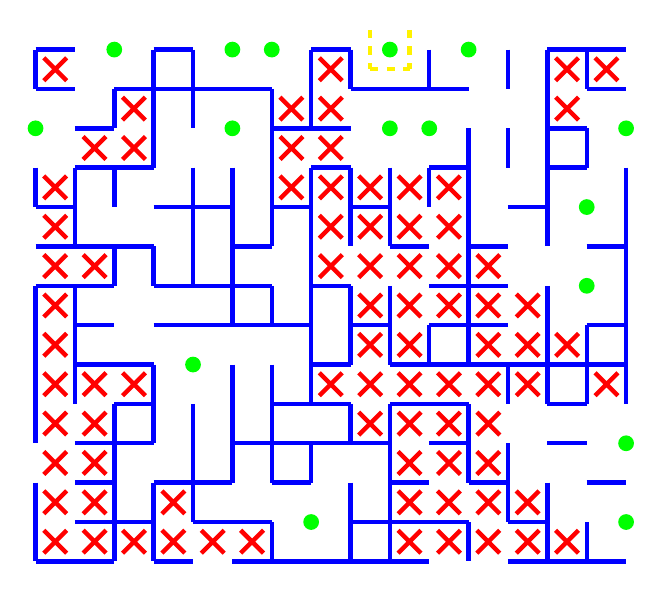
\begin{tikzpicture}[x=0.5cm, y=-0.5cm, ultra thick, blue]
% Walls
    \draw (0,0) -- (1,0);
    \draw (3,0) -- (4,0);
    \draw (7,0) -- (8,0);
    \draw (13,0) -- (15,0);
    \draw (0,1) -- (1,1);
    \draw (2,1) -- (6,1);
    \draw (8,1) -- (11,1);
    \draw (14,1) -- (15,1);
    \draw (1,2) -- (2,2);
    \draw (6,2) -- (8,2);
    \draw (13,2) -- (14,2);
    \draw (1,3) -- (3,3);
    \draw (7,3) -- (8,3);
    \draw (10,3) -- (11,3);
    \draw (13,3) -- (14,3);
    \draw (0,4) -- (1,4);
    \draw (3,4) -- (5,4);
    \draw (6,4) -- (7,4);
    \draw (8,4) -- (9,4);
    \draw (12,4) -- (13,4);
    \draw (0,5) -- (3,5);
    \draw (5,5) -- (6,5);
    \draw (9,5) -- (10,5);
    \draw (11,5) -- (12,5);
    \draw (14,5) -- (15,5);
    \draw (0,6) -- (2,6);
    \draw (3,6) -- (6,6);
    \draw (7,6) -- (8,6);
    \draw (10,6) -- (12,6);
    \draw (1,7) -- (2,7);
    \draw (3,7) -- (7,7);
    \draw (8,7) -- (9,7);
    \draw (10,7) -- (12,7);
    \draw (14,7) -- (15,7);
    \draw (1,8) -- (3,8);
    \draw (7,8) -- (8,8);
    \draw (9,8) -- (15,8);
    \draw (2,9) -- (3,9);
    \draw (6,9) -- (8,9);
    \draw (9,9) -- (11,9);
    \draw (13,9) -- (14,9);
    \draw (1,10) -- (3,10);
    \draw (5,10) -- (9,10);
    \draw (10,10) -- (11,10);
    \draw (13,10) -- (14,10);
    \draw (1,11) -- (2,11);
    \draw (3,11) -- (5,11);
    \draw (6,11) -- (7,11);
    \draw (9,11) -- (10,11);
    \draw (11,11) -- (12,11);
    \draw (14,11) -- (15,11);
    \draw (1,12) -- (3,12);
    \draw (4,12) -- (6,12);
    \draw (8,12) -- (11,12);
    \draw (12,12) -- (13,12);
    \draw (0,13) -- (2,13);
    \draw (3,13) -- (4,13);
    \draw (5,13) -- (10,13);
    \draw (12,13) -- (15,13);
    \draw (0,0) -- (0,1);
    \draw (0,3) -- (0,4);
    \draw (0,6) -- (0,10);
    \draw (0,11) -- (0,13);
    \draw (1,3) -- (1,5);
    \draw (1,6) -- (1,9);
    \draw (2,1) -- (2,2);
    \draw (2,3) -- (2,4);
    \draw (2,5) -- (2,6);
    \draw (2,9) -- (2,13);
    \draw (3,0) -- (3,3);
    \draw (3,5) -- (3,6);
    \draw (3,8) -- (3,10);
    \draw (3,11) -- (3,13);
    \draw (4,0) -- (4,2);
    \draw (4,3) -- (4,6);
    \draw (4,9) -- (4,12);
    \draw (5,3) -- (5,7);
    \draw (5,8) -- (5,11);
    \draw (6,1) -- (6,5);
    \draw (6,6) -- (6,7);
    \draw (6,8) -- (6,11);
    \draw (6,12) -- (6,13);
    \draw (7,0) -- (7,2);
    \draw (7,3) -- (7,9);
    \draw (7,10) -- (7,11);
    \draw (8,0) -- (8,1);
    \draw (8,3) -- (8,5);
    \draw (8,6) -- (8,8);
    \draw (8,9) -- (8,10);
    \draw (8,11) -- (8,13);
    \draw (9,3) -- (9,5);
    \draw (9,6) -- (9,8);
    \draw (9,9) -- (9,13);
    \draw (10,0) -- (10,1);
    \draw (10,3) -- (10,4);
    \draw (10,7) -- (10,8);
    \draw (11,2) -- (11,8);
    \draw (11,9) -- (11,11);
    \draw (11,12) -- (11,13);
    \draw (12,0) -- (12,1);
    \draw (12,2) -- (12,3);
    \draw (12,8) -- (12,9);
    \draw (12,10) -- (12,12);
    \draw (13,0) -- (13,5);
    \draw (13,6) -- (13,9);
    \draw (13,11) -- (13,13);
    \draw (14,0) -- (14,1);
    \draw (14,2) -- (14,3);
    \draw (14,7) -- (14,9);
    \draw (14,12) -- (14,13);
    \draw (15,3) -- (15,9);
% Pillars
    \fill[green] (2,0) circle(0.2);
    \fill[green] (5,0) circle(0.2);
    \fill[green] (6,0) circle(0.2);
    \fill[green] (9,0) circle(0.2);
    \fill[green] (11,0) circle(0.2);
    \fill[green] (0,2) circle(0.2);
    \fill[green] (5,2) circle(0.2);
    \fill[green] (9,2) circle(0.2);
    \fill[green] (10,2) circle(0.2);
    \fill[green] (15,2) circle(0.2);
    \fill[green] (14,4) circle(0.2);
    \fill[green] (14,6) circle(0.2);
    \fill[green] (4,8) circle(0.2);
    \fill[green] (15,10) circle(0.2);
    \fill[green] (7,12) circle(0.2);
    \fill[green] (15,12) circle(0.2);
% Inner points in accessible cul-de-sacs
    \node at (0.5,0.5) {};
    \node at (7.5,0.5) {};
    \node at (13.5,0.5) {};
    \node at (14.5,0.5) {};
    \node at (2.5,1.5) {};
    \node at (6.5,1.5) {};
    \node at (7.5,1.5) {};
    \node at (13.5,1.5) {};
    \node at (1.5,2.5) {};
    \node at (2.5,2.5) {};
    \node at (6.5,2.5) {};
    \node at (7.5,2.5) {};
    \node at (0.5,3.5) {};
    \node at (6.5,3.5) {};
    \node at (7.5,3.5) {};
    \node at (8.5,3.5) {};
    \node at (9.5,3.5) {};
    \node at (10.5,3.5) {};
    \node at (0.5,4.5) {};
    \node at (7.5,4.5) {};
    \node at (8.5,4.5) {};
    \node at (9.5,4.5) {};
    \node at (10.5,4.5) {};
    \node at (0.5,5.5) {};
    \node at (1.5,5.5) {};
    \node at (7.5,5.5) {};
    \node at (8.5,5.5) {};
    \node at (9.5,5.5) {};
    \node at (10.5,5.5) {};
    \node at (11.5,5.5) {};
    \node at (0.5,6.5) {};
    \node at (8.5,6.5) {};
    \node at (9.5,6.5) {};
    \node at (10.5,6.5) {};
    \node at (11.5,6.5) {};
    \node at (12.5,6.5) {};
    \node at (0.5,7.5) {};
    \node at (8.5,7.5) {};
    \node at (9.5,7.5) {};
    \node at (11.5,7.5) {};
    \node at (12.5,7.5) {};
    \node at (13.5,7.5) {};
    \node at (0.5,8.5) {};
    \node at (1.5,8.5) {};
    \node at (2.5,8.5) {};
    \node at (7.5,8.5) {};
    \node at (8.5,8.5) {};
    \node at (9.5,8.5) {};
    \node at (10.5,8.5) {};
    \node at (11.5,8.5) {};
    \node at (12.5,8.5) {};
    \node at (14.5,8.5) {};
    \node at (0.5,9.5) {};
    \node at (1.5,9.5) {};
    \node at (8.5,9.5) {};
    \node at (9.5,9.5) {};
    \node at (10.5,9.5) {};
    \node at (11.5,9.5) {};
    \node at (0.5,10.5) {};
    \node at (1.5,10.5) {};
    \node at (9.5,10.5) {};
    \node at (10.5,10.5) {};
    \node at (11.5,10.5) {};
    \node at (0.5,11.5) {};
    \node at (1.5,11.5) {};
    \node at (3.5,11.5) {};
    \node at (9.5,11.5) {};
    \node at (10.5,11.5) {};
    \node at (11.5,11.5) {};
    \node at (12.5,11.5) {};
    \node at (0.5,12.5) {};
    \node at (1.5,12.5) {};
    \node at (2.5,12.5) {};
    \node at (3.5,12.5) {};
    \node at (4.5,12.5) {};
    \node at (5.5,12.5) {};
    \node at (9.5,12.5) {};
    \node at (10.5,12.5) {};
    \node at (11.5,12.5) {};
    \node at (12.5,12.5) {};
    \node at (13.5,12.5) {};
% Entry-exit paths without intersections
    \draw[dashed, yellow] (8.5,0.5) -- (9.5,0.5);
    \draw[dashed, yellow] (8.5,-0.5) -- (8.5,0.5);
    \draw[dashed, yellow] (9.5,-0.5) -- (9.5,0.5);
\end{tikzpicture}
\end{center}
\vspace*{\fill}

\end{document}
